\section{System Design}
\subsection{Introduction}
The team \emph{Deadline Fighters} was given the overall requirement to build a ‘hub and spoke’ file synchroniser which has a single central server (the ‘hub’) to which multiple other clients (the ‘spokes’) can synchronise. The following are the operations that it entails and the priority of implementation we set for our team.

\bgroup
\def\arraystretch{1.3}
\begin{table}[H]
\centering
\begin{tabular}{|c|m{8cm}|}
\hline
Client name & User role\\
\hline
{Desktop and Mobile} & View files on the server \\ \cline{2-2}
& Upload a file from local which is outside the local sync folder (only for Android) \\
\cline{2-2}
& Upload a single file from local sync folder \\
\cline{2-2}
& Upload multiple files from local sync folder\\
\cline{2-2}
&Download a single file from server\\
\cline{2-2}
&Download multiple files from server\\
\cline{2-2}
&Reflect delete of a single file (Local to server)\\
\cline{2-2}
&Reflect delete of a single file (Server to local)\\
\cline{2-2}
&Reflect delete of multiple files (Local to server)\\
\cline{2-2}
&Reflect delete of multiple files (Server to local)\\
\cline{2-2}
&Reflect rename (Local to server)\\
\cline{2-2}
&Reflect rename (Server to local)\\
\cline{2-2}
&Download edited changes on a single file from server\\
\cline{2-2}
&Download changes on two or more files from server\\
\cline{2-2}
&Synchronize all server and local files\\
\hline
\bottomrule
\end{tabular}
\caption{Functionalities to be enabled on client applications}
\end{table}
\egroup

\bgroup
\def\arraystretch{1.2}
\begin{table}[H]
\centering
\begin{tabular}{|m{2cm}|m{2cm}|m{1.5cm}|m{2.5cm}|}
\hline
Operation & Object & Priority & Description \\
\hline
\multirow{2}{*}{Upload}&{One file (May not in the local sync folder)}&1&{Priority description:}\\
\cline{2-3}
&All files in the local sync folder&2&{\textbf{1-Highest priority}}\\
\cline{1-3}
\multirow{2}{*}{Download}&{One file}&1&{(Important /necessary functions)}\\
\cline{2-3}
&All files&2&{}\\
\cline{1-3}
\multirow{2}{*}{Delete}&{One file}&2&{\textbf{4-Lowest priority}}\\
\cline{2-3}
&All files&3&{}\\
\cline{1-3}
\multirow{2}{*}{Rename}&{One file}&2&{(Will implement if time permits)}\\
\cline{2-3}
&Two or more files&3&{}\\
\cline{1-3}
\multirow{2}{*}{Edit}&{One file}&4&{}\\
\cline{2-3}
&Two or more files&4&{}\\
\cline{1-3}
\multirow{1}{*}{Synchronize}&{All files in the server and local sync folder}&2&{}\\
\cline{1-4}
\bottomrule
\end{tabular}
\caption{Priority of operations to be implemented on client applications}
\end{table}
\egroup

\subsection{Architecture}

\begin{figure}[h!]
\centering
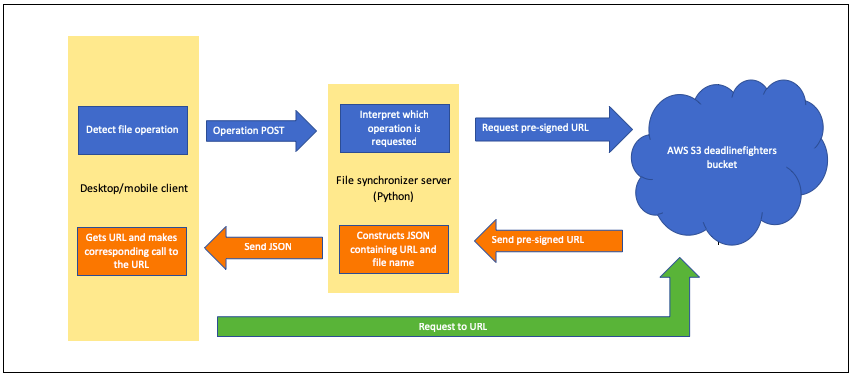
\includegraphics[scale=0.5]{Architecture}
\caption{Flow of operation across client, server and AWS S3}
\end{figure}


\subsection{Central server’s conflict role}
For central server: it will solve the conflict between multiple users operate at same time. The operate and resolution is shown as follow table.\newline
(Add conflict table here.)\newline
By using the conflict role as above in the file synchronisation tool development allows the system to reduce the number of error reports and make the system organized. It won't cause the system to lose files and report error when the user using two different synchronization functions at the same time to the server (eg. A client edit a file on the desktop application and the client delete the file on the mobile at the same time). It can avoid unnecessary data losses. Because the most important thing about a synchronous system is that you can't lose files. Through the table listed above, our team group can have a common standard for dealing with conflicts in the development process, making the development process more organized.\newline
According to the above detailed requirements design and contradictory solutions, it can help our team have a better assignment for the tasks to the team members and promote the teamwork. Team members can arrange their own time according to their own tasks to complete system functions implementation.\newline

